\chapter{Btqw - Queue Management Tool}
\label{chp:btqw}

\includegraphics{img/win2.png} 

\progname{Btqw} is a Microsoft Windows Client alternative to the
standard batch queue manager, \PrBtq. It is usually
invoked from the Windows Program Manager, or from the desktop by
clicking on the \progname{Btqw} icon shown above.

\section{The Main Window}
When \progname{btqw} is invoked the main window will be
displayed, with a sub-window for jobs. By default it will look
something like this:

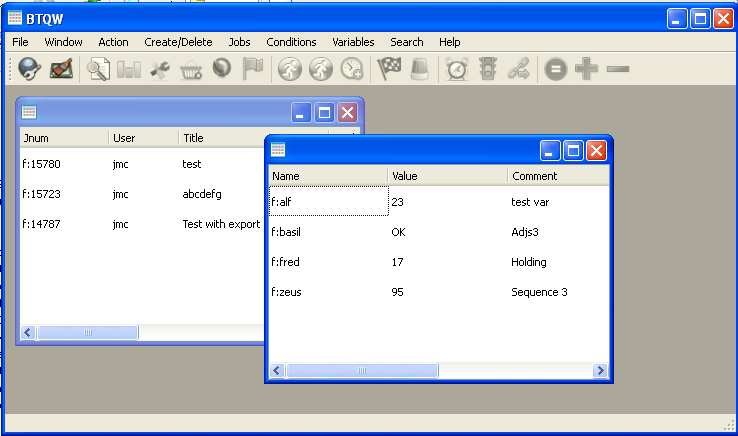
\includegraphics{img/btqwjwfirst.png} 

The main window has two key functional areas. The top area contains
menus and short cut buttons for issuing commands. The larger, bottom
area, holds the sub-windows for batch jobs and variables. These may be
selected to have commands performed upon them.

Like with other Windows applications the windows may be moved, resized, maximised and minimised.

Menu options allow the windows to be tiled horizontally and vertically or cascaded.

The widths of each column in each of the windows may be adjusted as required by dragging across the border. Alternatively double-clicking
on the border will fit the width of the column to the largest field displayed.

The user can have any number of job and variable windows and specify different jobs or variables
selected by various criteria in each and also different attributes of the jobs and variables
in each.

When \progname{btqw} is exited, the current selections and sizes for each window are saved
and are restored when it is restarted.

If a menu option or button is ``greyed out''
it means that a suitable job or variable has not been selected. It may
be that the required item is selected but not the sub-window that
contains it. Look at the ``title bar'' of the
sub-window to see if it is the ``active window''.

\section{The Menus and Shortcut Buttons}
All commands are performed by selecting a menu option or clicking on the
equivalent shortcut button. Some of the menu options may also be
selected using shortcut keys, which are indicated to the right of the
relevant options in each menu.

Other options may be selected from a ``right-click'' popup menu from the appropriate place
on a job or variable window.

\subsection{The File Menu}
The file menu selects various global options, notably the server list.

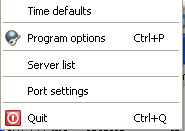
\includegraphics{img/btqwfilemenu.png} 

\textbf{Time defaults} opens a dialog for setting default time
and repeat specifications for jobs. This is separate from the defaults used by
\progname{btrw}.

\textbf{Program options} brings up the Program options dialog, to tailor
the look and feel of \progname{btqw}.

\textbf{Server list} maintains the list of servers to which \progname{btqw}
and \progname{btrw} communicate.

\textbf{Port settings} enables the TCP ports on which \progname{btqw} and
\progname{btrw} communicate with the servers to be adjusted.

\textbf{Quit} quits \progname{btqw}.

The following shortcut button is provided on the toolbar.

\begin{tabular}{l p{12cm}}

\includegraphics{img/btqwprogopts.png} & is a shortcut button for \textbf{Program options}.\\
\end{tabular}

\subsection{The Window menu}
For opening new job and variable list windows, changing the layout of
windows and formatting their contents.

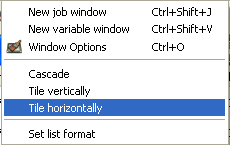
\includegraphics{img/btqwwinmenu.png} 

\textbf{New Job Window} opens a new window containing a Job List.

\textbf{New Variable Window} opens a new window containing a Variable
List.

\textbf{Window Options} sets a filter to be applied to the currently-selected job
or variable window to limit the jobs or variables displayed to those matching
given criteria. The filter set is saved and restored separately for each window
across \progname{btqw} sessions.

\textbf{Cascade}, \textbf{Tile Horizontally} and \textbf{Tile Vertically} re-arrange the job and variable windows
in standard ways.

\textbf{Set list format} Adjusts which attributes of each job or variable are to be displayed in the
currently-selected window. This information is saved across \progname{btqw} sessions.

The following shortcut button is provided on the toolbar.

\begin{tabular}{l p{12cm}}

\includegraphics{img/btqwwinopts.png} & Is a shortcut button for \textbf{Window Options}\\
\end{tabular}

\subsection{The Action Menu}
For high level actions: starting and stopping batch jobs.

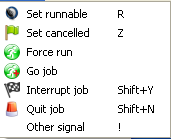
\includegraphics{img/btqwactmenu.png} 

\textbf{Set runnable} will change a job from the \textit{Cancelled},
\textit{Error} or \textit{Abort} state to the \textit{Ready} or
\textit{Run} state. This option is also available using the shortcut
button.

\textbf{Set cancelled} puts a job on held (i.e. not able to run). This
option is also available using the `Set cancelled' shortcut button.

\textbf{Force run} sets a job runnable and overrides any time
specification to allow the job to run as soon as any Variable
Conditions are satisfied. This option is also available using the
`Force run' shortcut button.

\textbf{Go job} sets a job runnable overriding any time specification to
allow the job to run as soon as any Variable Conditions are satisfied.
The repeat time on the job is advanced to the next repetition. This
option is also available using the `Go Job' shortcut button.

\textbf{Interrupt job} attempts to terminate a running job by sending it
an Interrupt Signal. This option is also available using the
`Interrupt job' shortcut button and by clicking the right mouse button over the job to select it and
selecting ``kill'' from the pop-up menu.

\textbf{Quit job} tries to terminate a running job with a Quit Signal.
This option is also available using the `Quit job' shortcut button.

\textbf{Other signal} attempts to terminate a running job by sending it
a specified Signal. This option opens a selection dialog to choose which signal to send.

The following shortcut buttons are provided on the toolbar.

\begin{tabular}{l p{12cm}}

\includegraphics{img/btqwsetrun.png} & Is a shortcut for \textbf{Set runnable}\\

\includegraphics{img/btqwsetcanc.png} & Is a shortcut for \textbf{Set cancelled}\\

\includegraphics{img/btqwforcerun.png} & Is a shortcut for \textbf{Force run}\\

\includegraphics{img/btqwgojob.png} & Is a shortcut for \textbf{Go job}\\

\includegraphics{img/btqwintjob.png} & Is a shortcut for \textbf{Interrupt job}\\

\includegraphics{img/btqwquitjob.png} & Is a shortcut for \textbf{Quit job}\\
\end{tabular}

\subsection{Create/delete menu}
This menu offers options for creating and deleting variables, deleting jobs and an option to invoke a copy of \progname{btrw} to create
jobs (although you may prefer to invoke it via the desktop icon). It also offers options to change job and variable permissions.

Depending on whether a job or variable window is selected, the inappropriate menu items are greyed out. The version below is that
applicable if a job window is selected.

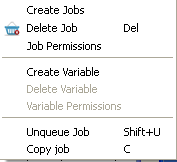
\includegraphics{img/btqwcredelmenu.png}

\textbf{Create jobs} invokes a copy of \progname{btrw}.

\textbf{Delete job} deletes the currently-selected job. Depending on the setting of the delete confirmation option in the
Program Options dialog, confirmation may or may not be requested.

\textbf{Job Permissions} displays and provides options to set the permissions on the currently-selected job.

\textbf{Create variable} creates a new variable on a server.

\textbf{Delete variable} deletes the currently-selected variable.

\textbf{Variable Permissions} displays and provides options to set the permissions on the currently-selected variable.

\textbf{Unqueue} removes the job from the queue, putting a copy on the PC hard disk possibly for editing and re-submission using
\progname{btrw}.

\textbf{Copy job} takes a copy of the job from the queue, putting the copy on the PC hard disk possibly for editing and re-submission using \progname{btrw}. The original job is left on the queue unchanged.

The following shortcut button is provided on the toolbar.

\begin{tabular}{l p{12cm}}

\includegraphics{img/btqwdeljob.png} & Is a shortcut for \textbf{Delete job}\\
\end{tabular}

\subsection{Jobs menu}
This menu provides options for displaying and modifying attributes of jobs.

Note that the items here will be greyed out unless a job in a job window is selected.

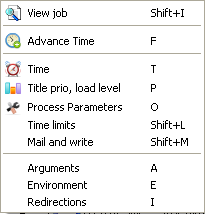
\includegraphics{img/btqwjobsmenu.png}

\textbf{View job} opens a text browser showing the job script to be run. This can also be selected by using the `View
job' shortcut button and by right-clicking the mouse over the job on the job list and selecting the option from the pop-up
menu.

\textbf{Advance Time} skips the next scheduled execution of a job by advancing to the next repetition. This option is also available using
the `Advance Time' shortcut button.

\textbf{Time} brings up a dialog for setting the start time, retention options, repetition details and list of days to avoid.
This option is also available using the `Time' shortcut button.

\textbf{Title prio, load level} brings up the dialog to set the job title, priority, load level and command interpreter.

\textbf{Process parameters} brings up the dialog to select the process parameters: working directory, ulimit, umask, network scope and which
exit codes represent an error.

\textbf{Time limits} opens the dialog for specifying time restrictions to terminate a runaway job.

\textbf{Mail and write} opens the dialog to specify what notification is required when a job finishes.

\textbf{Arguments} opens a dialog for adding, modifying and deleting arguments that are passed to the job on its command line.

\textbf{Environment} opens a dialog for adding, editing and deleting the environment variables in the jobs run time environment.

\textbf{Redirections} opens the dialog for specifying I/O redirections.

The following shortcut buttons are provided on the toolbar.

\begin{tabular}{l p{12cm}}

\includegraphics{img/btqwviewjob.png} & Is a shortcut for \textbf{View Job}\\

\includegraphics{img/btqwadvtime.png} & Is a shortcut for \textbf{Advance Time}\\

\includegraphics{img/btqwtimeset.png} & Is a shortcut for \textbf{Time}.\\

\includegraphics{img/btqwtitprill.png} & Is a shortcut for \textbf{Title Priority Load Level}.\\

\includegraphics{img/btqwprocpar.png} & Is a shortcut for \textbf{Process Parameters}.\\
\end{tabular}

\subsection{The Conditions Menu}
Provides options for setting up pre-conditions and assignments.

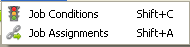
\includegraphics{img/btqwcondsmenu.png} 

\textbf{Job conditions} brings up the dialog to add, modify and delete
pre-conditions on the selected batch job.

\textbf{Job assignments} brings up the dialog to add, modify and delete
assignments for the selected batch job.

Both these options are available using the toolbar buttons shown.
Additionally a job may be selected and one these options set by
right-clicking the mouse over the relevant job on the job list and
selecting from the pop-up menu.

The shortcut buttons are:

\begin{tabular}{l p{12cm}}

\includegraphics{img/btqwcond.png} & For \textbf{Job Conditions}\\

\includegraphics{img/btqwass.png} & For \textbf{Job Assignments}\\
\end{tabular}

\subsection{The Variables Menu}
Provides options for manipulating variables.

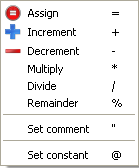
\includegraphics{img/btqwvarmenu.png} 

\textbf{Assign} brings up the dialog to modify the
data held by the selected variable. This option is also available on
the tool-bar button and on the right-click pop-up menu.

\textbf{Increment} increments the value of the selected variable by the
currently set constant. This option is also available on the tool-bar
button and on the right-click pop-up menu.

\textbf{Decrement} decrements the value of the selected variable by the
currently set constant. This option is also available on the tool-bar
button and on the right-click pop-up menu.

\textbf{Multiply }multiplies the value of the selected variable by the
currently set constant.

\textbf{Divide }divides the value of the selected variable by the
currently set constant.

\textbf{Remainder} performs a modulo on the value of the selected
variable by the currently set constant.

\textbf{Set comment} brings up the dialog to modify the comment field of
the selected variable. This option is also available on the right-click
pop-up menu

\textbf{Set constant} for the increment, subtract, multiply, divide and
remainder operations. This option is also available on the right-click
pop-up menu.

The following shortcut buttons are provided on the toolbar.

\begin{tabular}{l p{12cm}}

\includegraphics{img/btqwvass.png} & Is a shortcut for \textbf{Assign}\\

\includegraphics{img/btqwvincr.png} & Is a shortcut for \textbf{Increment}\\

\includegraphics{img/btqwvdecr.png} & Is a shortcut for \textbf{Decrement}\\
\end{tabular}

\subsection{The Search Menu}
Both the variable and job lists may be navigated by using search options
to find an item of interest.

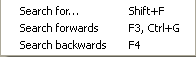
\includegraphics{img/btqwsearchmenu.png} 

\textbf{Search for} a specified item or pattern.

\textbf{Search forward} from the current position

\textbf{Search backward} from the current position

\subsection{Help}
Help for using \progname{btqw}.


\includegraphics{img/btqwhelpmenu.png} 

\textbf{About} displays information, such as release number, about the
version of \progname{btqw} that is running.

\subsection{Pop-up menus}
Jobs and variables may be selected and various commonly-selected options
applied by right-clicking on the job or variable list, usually on the job or variable to be accessed. This will select
the job or variable clicked over and bring up pop-up menus.

For jobs the pop-up menu is as follows:

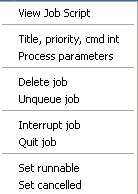
\includegraphics{img/btqwjobpop.png}

For variables the pop-up menu is as follows:

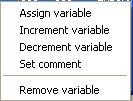
\includegraphics{img/btqwvarpop.png}

\section{Dialogs}
Much of the contents of the \progname{btqw} dialog boxes are similar to those in other \ProductName{} interfaces,
however for completeness some additional details and explanations are provided here.

\subsection{Program Options}
The \textbf{Program Options} dialog in the \textbf{File} menu provides some options relating to the whole program.

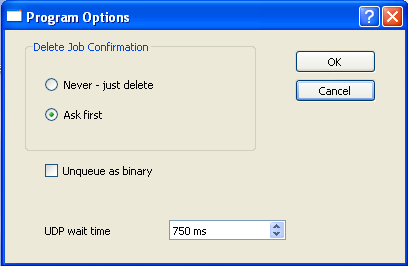
\includegraphics{img/btqwprogoptsdlg.png}

\subsubsection{Setting the Confirmation level}
By default \progname{btqw} asks for confirmation before deleting any job from the
queue. This may be relaxed to allow jobs to be deleted without
confirmation if required by selecting the radio button.

Note that this applies to all windows.

\subsubsection{Unqueue as binary}
If this option is selected no conversions on MS Windows are done to insert carriage return characters
in front of linefeed characters when the job is unqueued.

\subsubsection{UDP wait time}
Certain operations (login and similar) are carried out by means of UDP messages. This option selects how long a
response will be awaited in each case.

\subsection{Server list}
The server list dialog was mentioned in the installation on page \pageref{bkm:installservs}, and looks like this.

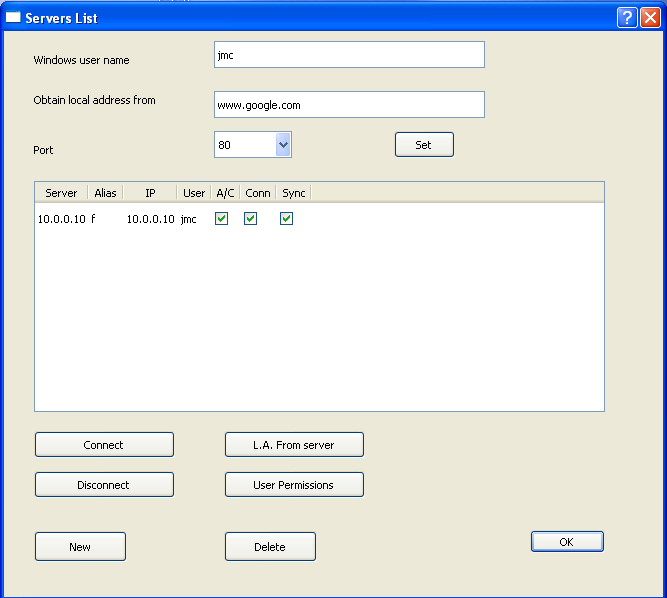
\includegraphics{img/btqwnewhostsetlist.png}

The function of this dialog is to set up and maintain the list of servers running \ProductName{} to which \progname{btqw}
(and also \progname{btrw} communicates and to possibly connect and disconnect them.

Particularly important is that the client can obtain its own address quickly and the usual convention is to put a
website which it can connect to and extract its own local IP address from there.

Alternatively a client can interrogate a server by selecting it and pressing the \textbf{L.A. from server} button.

The \textbf{User Permissions} button displays the permissions which the user has on the server, including
the user and group names assigned.

\section{Window Options}

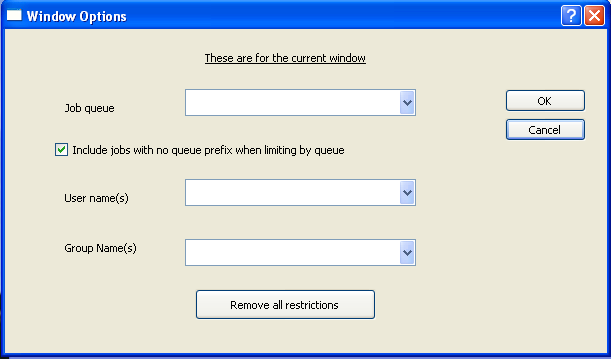
\includegraphics{img/btqwwinoptsdlg.png}

This dialog applies some options to the current window to curtail jobs or variables in which the user has no
interest. THe limitation applies until it is changed and is saved when \progname{btqw} is quit. Initially no restrictions
are set.

The Job queue restriction applies to jobs, but the other restrictions apply to both jobs and variables.

Sets of queues, users or groups may contain just one name, a list of names or a
list of patterns for matching names. The group and user names may be
given as a comma-separated list of alternatives, including the use of
shell-style wild-cards. For example

\begin{expara}

fred

jmc,tony,ukops\_jmc,ukops\_wal

ukops*,ukadmin[1-5]

\end{expara}

The wild-card options are:

\begin{center}
\begin{tabular}{l l}
\exampletext{*} & Matches anything\\
\exampletext{?} & Matches one character\\
\exampletext{[a-m]} & Matches one character in list or range\\
\exampletext{[!n-z]} & Matches one character not in list or range\\
\end{tabular}
\end{center}

If only one explicit name is required, the drop-down combo box may be used to select it.

To remove all the restrictions quickly, press the button.

\section{Changing the fields displayed}
If you want to change which attributes of jobs or variables are displayed in a given
window, you can select the menu entry \textbf{Set list format} in the \textbf{Window}
menu.

For a job window with default settings, the following dialog is displayed.

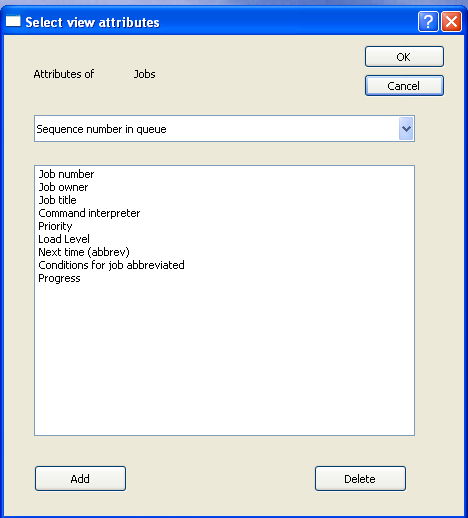
\includegraphics{img/btqwjlistfmt.png}

The equivalent for a variable window is.

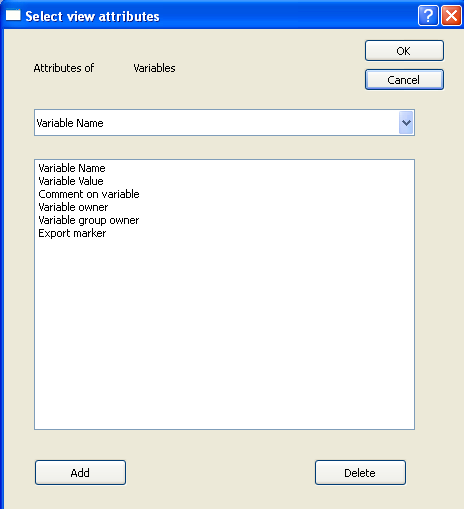
\includegraphics{img/btqwvlistfmt.png}

Each row on the list of attributes corresponds to a column on the displayed window.

To add a new attribute to display, select it from the drop-down box at the top and click the \textbf{Add} button.

To delete an attribute, select it and press the \textbf{Delete} button.

The fields can be reordered by dragging and dropping.

The selected fields are specific to the window being displayed and are saved and restored for when \progname{btqw} is re-entered.

On the window display the column widths can be adjusted by dragging the borders. Double-clicking on the border will set the width of the
current column to the widest entry displayed. The widths are also saved and restored across \progname{btqw} sessions.

